\documentclass[12pt]{report}
\usepackage[utf8]{inputenc} 
\usepackage[T1]{fontenc}
\usepackage[francais]{babel}
\usepackage{layout}
\usepackage{graphicx}

%page de garde 
\title{Report of the first Phase of the project}
\author{Pierre-Yves \bsc{Hervo} \\Polytech Nantes High school of Engineering }
\date{11\up{th} of July 2013}

\begin{document}
\maketitle

\begin{abstract}

The ICCMR laboratory is a structure which deals with sounds and one of their field of research is the Human voice. In this perspective, they launched a project to design a software which can synthesis human voice by giving it formants values. This is big project which had been divided into smaller ones and which will be improve at each step. I worked on the first step of the project, the launch of the project which consisted in developing a JAVA software to recreate vowels. 

In this report, I will explain the interest of this project and the work I have realised on the first part.
\paragraph{}
NOTE ; This report presents the work I have realised on my project from the beginning of my internship the 03\up{rd} of June to the end of the first Phase the 12\up{th}of July.

\end{abstract}

\renewcommand{\contentsname}{Sommaire}
\tableofcontents

J'insère le premier \cite{ref}  \cite{ref2} \cite{ref3} \cite{ref4}


\part{Overall}
\chapter{Presentation of the project}
\section{Quick introduction}
As I said in the introduction, i worked on the first phase of the global project by designing and developing a software that is capable of recreating the human vowels.
But what is the purpose of this project and why do I only worked on vowels ?
Isn't there existing software to synthesise human sound ?
\paragraph{}
Before giving the answer I had to make a little recap on the voice synthesis
 
\section{Presentation of Voice Synthesis}
We will here study the human voice from a physical point of view.

The human voice are created by the combination of different organs in our body.
It started in the lungs by producing an airstream and then pass through different elements of the body to exit by the mouth. Among those elements we can quote for example the larynx, the vocal cords, the tongue, and so on...

Some of them are are represented in the Figure \ref{ImageHumanVoice} in the page \pageref{ImageHumanVoice}.


According to the position of this muscles, the sound produced will be different. For example if the vocal are tense or not, it will have an influence of the vibration of the voice and so on the sound. It is the same for all the organs previously described, the form they had during the passage of the airstream will have an impact on the final sound.

\begin{figure}
\begin{center}
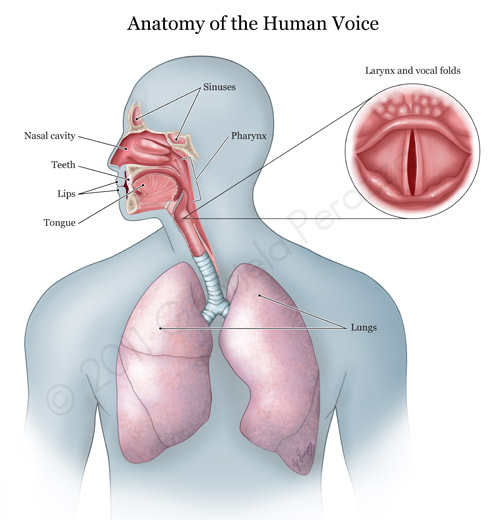
\includegraphics[scale=0.5]{resources/human_voice.jpg} 
\end{center}
\caption{Some of the organs use in the voice synthesis process}
\label{ImageHumanVoice}
\end{figure}

There is some software that allows to synthesis voice by given parameters that represents the state of those different elements. Among them, Praat \cite{ref1} is the most advanced.
It is the software that we will use for this project. We will present it in detail in another part of this report.

\section{The goal of the project}
The question that comes to mind is something like that already exists, why this project ?
In fact praat allow to synthesise human voice and the sound you wants if you know the value of the parameters. There is a lot of variables (near 50) and a wide range of possible values for each. So it is hard to determine which parameters send for which sound. The only way you have is to try values after values. You can be helped by your knowledge about the state of the elements for a particular sound. For example, in singing, folds are brought close together so you can guess it will be in a certain range of values in praat.

It is nearly impossible for long sound or it would take a long time. That 's why the ICCMR created this project. We will use Genetic algorithms to determinate the values for praat. This way we will avoid to search in the complete research space and so win time by using our knowledge to restrain the search space.

\section{Why vowels ?}
Because of the time allow to my project, i could only work for vowels. Vowels get particular formant values and so it is a firs step for the project.They are used a lot in long sounds.

\chapter{Presentation of Genetic algorithms}

\chapter{Presentation of Praat}

\part{Technical details}
\chapter{Praat Scripts}
\chapter{Presentation of watchmaker}
\chapter{Presentation of the basic manipulated Structures}
\chapter{result}
\appendix
\chapter{A scheme}

\listoffigures
\listoftables

\bibliographystyle{unsrt} 
\bibliography{bib} % mon fichier de base de données s'appelle bibli.bib
\end{document}